% 02-methods.tex

% Section Title
\section{METHODS} \label{sec:methods}

    \subsection{Devices and Software}
    
        We used a Samsung Galaxy A51 with Android 13 for this experiment.
        GNSS Logger v3.1.0.4~\cite{GNSSLogger2025} was chosen due to its unrestricted access to raw GNSS measurements, compatibility with newer Android APIs, and ability to record detailed GNSS data that is suitable for precise analysis.
        MATLAB R2024b~\cite{MATLAB2024b} was employed to handle data because it comes with Google's GNSS toolbox~\cite{GnssAnalysisTools2025}, which accommodates robust analysis and visualization of GNSS measurements and position solutions.
        
    \subsection{Data Collection Procedure}
    
        Two distinct 5-minute GNSS data logging sessions were conducted on 3 May 2025, under cloudy weather conditions, using the GNSS Logger app configured with the following settings enabled:

        \begin{itemize}
            \item \textbf{GNSS Location:} to capture location data.
            \item \textbf{GNSS Measurements:} to log raw GNSS measurements.
            \item \textbf{Navigation Messages:} to capture navigation data.
            \item \textbf{GnssStatus:} to log GNSS status information.
            \item \textbf{Sensors:} to capture sensor data.
        \end{itemize}
        
        \noindent The sessions were designed to capture both static and dynamic GNSS performance, with the following details:

        \begin{enumerate}[label=\alph*)]
            \item \textbf{Static Scenario:} performed on the viewpoint of \textit{Monte dei Cappuccini, Turin}, starting at 10:35:20. The device was stationary throughout the entire session, providing baseline measurements.
            \item \textbf{Dynamic Scenario:} conducted on tram line 15 from \textit{Piazza Castello} to \textit{Piazza Vittorio Veneto}, starting at 10:00:21, simulating a typical urban mobility scenario.
        \end{enumerate}

        \vspace{-0.5cm} % TODO: check

        \begin{figure}[h!]
            \centering
            \begin{subfigure}{0.23\textwidth}
                \centering
                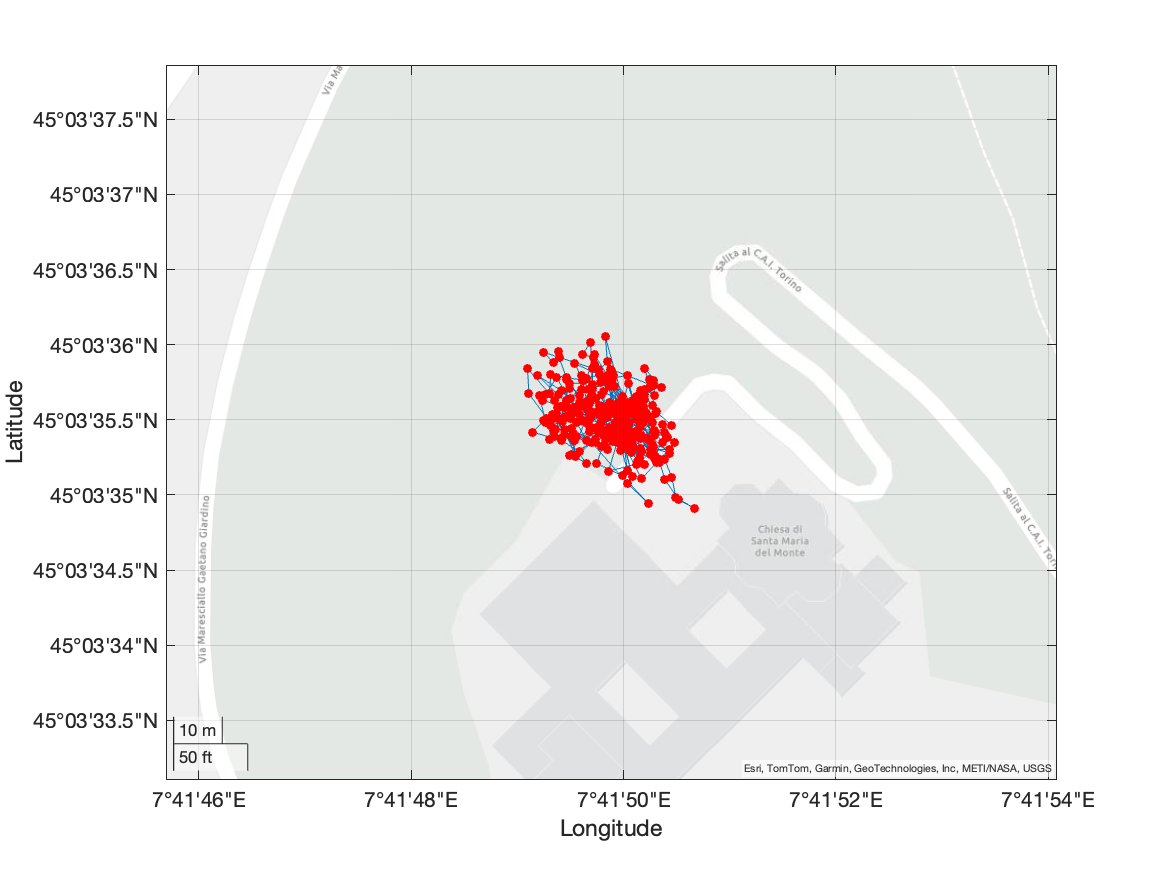
\includegraphics[width=\textwidth]{images/tests/Monte_Cappuccini/png/Samsung_A51_Monte_Cappuccini_fig6.png}
                \caption{Monte dei Cappuccini.}
                \label{fig:static_scenario}
            \end{subfigure}
            \hfill
            \begin{subfigure}{0.23\textwidth}
                \centering
                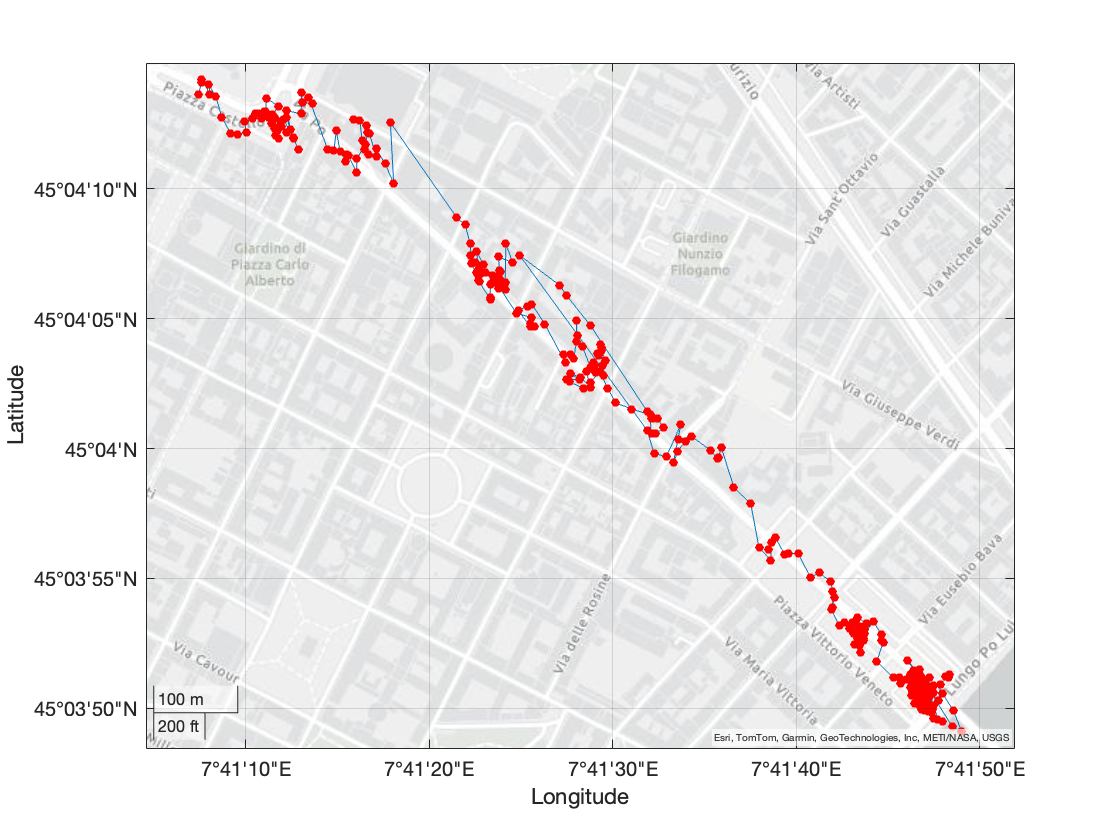
\includegraphics[width=\textwidth]{images/tests/Tram_15_trip_Castello_to_Pescatore/filtered/Samsung_A51_Tram_15_trip_Castello_to_Pescatore_fig6.png}
                \caption{Tram Line 15.}
                \label{fig:dynamic_scenario}
            \end{subfigure}
            \vspace{0.35cm}
            \caption{Comparison of GNSS data: static (a) and dynamic (b) scenarios.}
            \label{fig:gnss_comparison}
        \end{figure}

    \vspace{-0.2cm}

    \subsection{Processing Pipeline}
    
        The raw GNSS data from the GNSS Logger served as the input dataset for MATLAB. 
        Processing involved a scripted workflow via \cooltext{ProcessGnssMeasScript.m}~\cite{LabGNSSRepo}
        %\footnote{\url{https://github.com/WDCSecure/LabGNSS/blob/main/Lab-Material/scripts/matlab/core/ProcessGnssMeasScript.m}}
        , where the following steps were executed:

        \begin{enumerate}
            \item \textbf{Filtering:} data points not meeting predefined quality thresholds, such as signal strength or satellite geometry, were excluded to improve accuracy.
            \item \textbf{Measurement Extraction:} pseudorange and Doppler measurements were computed from GNSS timestamps and satellite transmission data.
            \item \textbf{Weighted Least Squares (WLS) Positioning:} applied to derive precise positioning and clock bias estimates.
            \item \textbf{Visualization and Comparison:} output plots from MATLAB, including pseudorange, pseudorange rates, and position solutions, were generated to facilitate comparative analysis of the static and dynamic scenarios.
        \end{enumerate}

        % \noindent Results from this processing pipeline provided insights into the differences in GNSS performance under static and dynamic conditions.
    
    \vspace{-0.1cm}

    \subsection{Spoofed-Input Configuration}

        Spoofing scenarios were emulated by introducing artificial variations to the recorded GNSS data through MATLAB processing. 
        Specifically, mock positions were assigned by adjusting the parameter \cooltext{spoof.position}, which represents modified latitude, longitude, and altitude coordinates. 
        Additionally, artificial time delays were tested by adjusting the \cooltext{spoof.delay} parameter, typically in milliseconds, to mimic delayed GNSS signal arrival, and \cooltext{cfg.t\_start} parameter to make the spoofed signal appear some seconds after the start of the session.
        Such configurations facilitated evaluation of the impact of spoofing scenarios on position estimation reliability and accuracy.

    % \vspace{-0.1cm}

    \subsection{Interference Scenario}
    
        The experimental setup involved enclosing a smartphone within three layers of aluminum foil while simultaneously exposing it to nearby sources of electromagnetic interference, including two active smartphones engaged in a call and multiple Bluetooth-enabled devices. 
        This configuration created a non-ideal environment for GNSS signal reception. %, where both intentional signal attenuation (via the aluminum shield) and unintentional radio-frequency (RF) noise coexisted. 
        The aluminum enclosure acted as a rudimentary Faraday cage, partially obstructing direct line-of-sight between the device's antenna and GNSS satellites, thereby weakening incoming signals. 
        Concurrently, the proximity of active communication devices introduced broadband RF interference, likely overlapping with GNSS frequency bands and degrading signal quality further.
